Before diving into the architectural details of the system, we first present a state of the art summary, that concisely describes what is the positioning of this project in light of the previous explored \glspl{sna} tools that we presented in Chapter 4, and also considering the \glspl{osn} that we study in Chapter 3.\\
\indent Specifically regarding the \glspl{sna} tools, we will comment some of them, some of their useful features and overall comments to what may lack on this tools that this project may target, in order to differentiate and not only \textit{''reinvent the wheel''}.\\

\section{Simplicity}
Aside of \textbf{Vizster} (\cite{heer2005vizster}), the majority of the previously presented tools such as Gephi \cite{bastian2009gephi} or Social Network Visualizer \cite{socnetv}, are very complex tools with very heavy interfaces, that have a big learning and are meant for users that have particular advanced knowledge in \glspl{sn} and \glspl{sna}. The tool to be developed could also serve for less expert users, providing a set of core basic functionalities (e.g only allow users to load and visualize they're networks), and then, allow the user to build complexity from there enabling and disabling other features.

\section{Accessibility}
All the software that we presented above exists in the form of desktop applications. This applications need to be downloaded, and installed in a compatible machines (sometimes with dependencies on other software that is not installed by default). Nowadays almost every application is web based, this allows users to access them every where trough a browser, making web apps a solution that is Operating System and device agnostic. This said, building a web based social networks analysis tool could be a way of tackle the accessibility of such tools.\\
\indent A web based application, it's good for sake of accessibility but in another hand it is a performance culprit when it comes to performance. This is a decision to take into account, but always having in mind that tackling performance it's not the main goal this master's thesis, also, the mentioned tools are mature projects that are highly performant and are capable of rendering huge networks.

\section{\acrfull{osn} integration}
Social Network Visualizer \cite{socnetv}, allows to \textit{scrap} web sites to build networks, but for this feature relays only on links to build the network (it blindly scraps recursively some url to build the network). By allowing the user the power to the user to analyze networks that are directly reporting they're social network status would be a differentiation factor from the other tools, and would certainly be a more meaningful and valuable analysis for the end user.

\section{Drawing Accurate Conclusions}
As we state before when talking about simplicity, the mentioned \glspl{sna} tools provide generic metrics on networks such as network density or actor centrality. The values outputted from this tools are the result of running generic formulas and algorithms against some networks, so its very common for current \glspl{sna} researchers to be worried about the size of the network, being their focus on \textbf{quantitive analysis}.\\
\indent In a hypothetical analysis scenario where some researcher has a network with a few thousand nodes, \textbf{what is the meaning of his assumptions when analyzing the network}? Since this is a pure quantitive analysis the numbers will seem reasonable for the given network, but this will not allow him to extract contextual conclusions, because in this case analyzing data form Facebook or analyzing data from LinkedIn will sound just like the same, because deep down it all comes down to the network. A better approach for drawing conclusions would be to have a mixture between \textbf{quantitive analysis} and \textbf{quality analysis}, the tool could do some content and context analysis to help the end user to get a more meaningful conclusion rather than just simple metrics.

% LOOK TO ME IF YOU WANT TO CLARIFY THIS IN THE FUTURE
% One thing that I see far to little of is a clever and reasonable combination of qualitative and quantitative data. Often SNA
% researchers will collect a lot of (quantitative) data about the links between the actors and calculate all kinds of amazing
% network and actor centrality measures and then basically make up the meaning of those by using their own assumptions. Let's
% say Vladis Krebs claimed that power in a network is where actors have high betweenness centrality (control) and closeness
% centrality (access). That sounds great and makes sense in theory. But when I combine (quantitative) network mapping with
% (qualitative) discussion of the meaning and an additional independent measure of influence, I find some actors influential
% because of their network position and others influential because of other factors. By adding the influence measure and
% discussion I get to really understand what the centrality measures mean in this specific context. If you are interested in the method I use for this:

\section{System Architecture}

Now, after building up our aiming for this project, we now present a more concrete image of the overall system. In Figure \ref{img:architectureprop} we present an abstract system architecture.

\begin{figure}[h!]
\begin{center}
  \hspace*{-0.3in}
  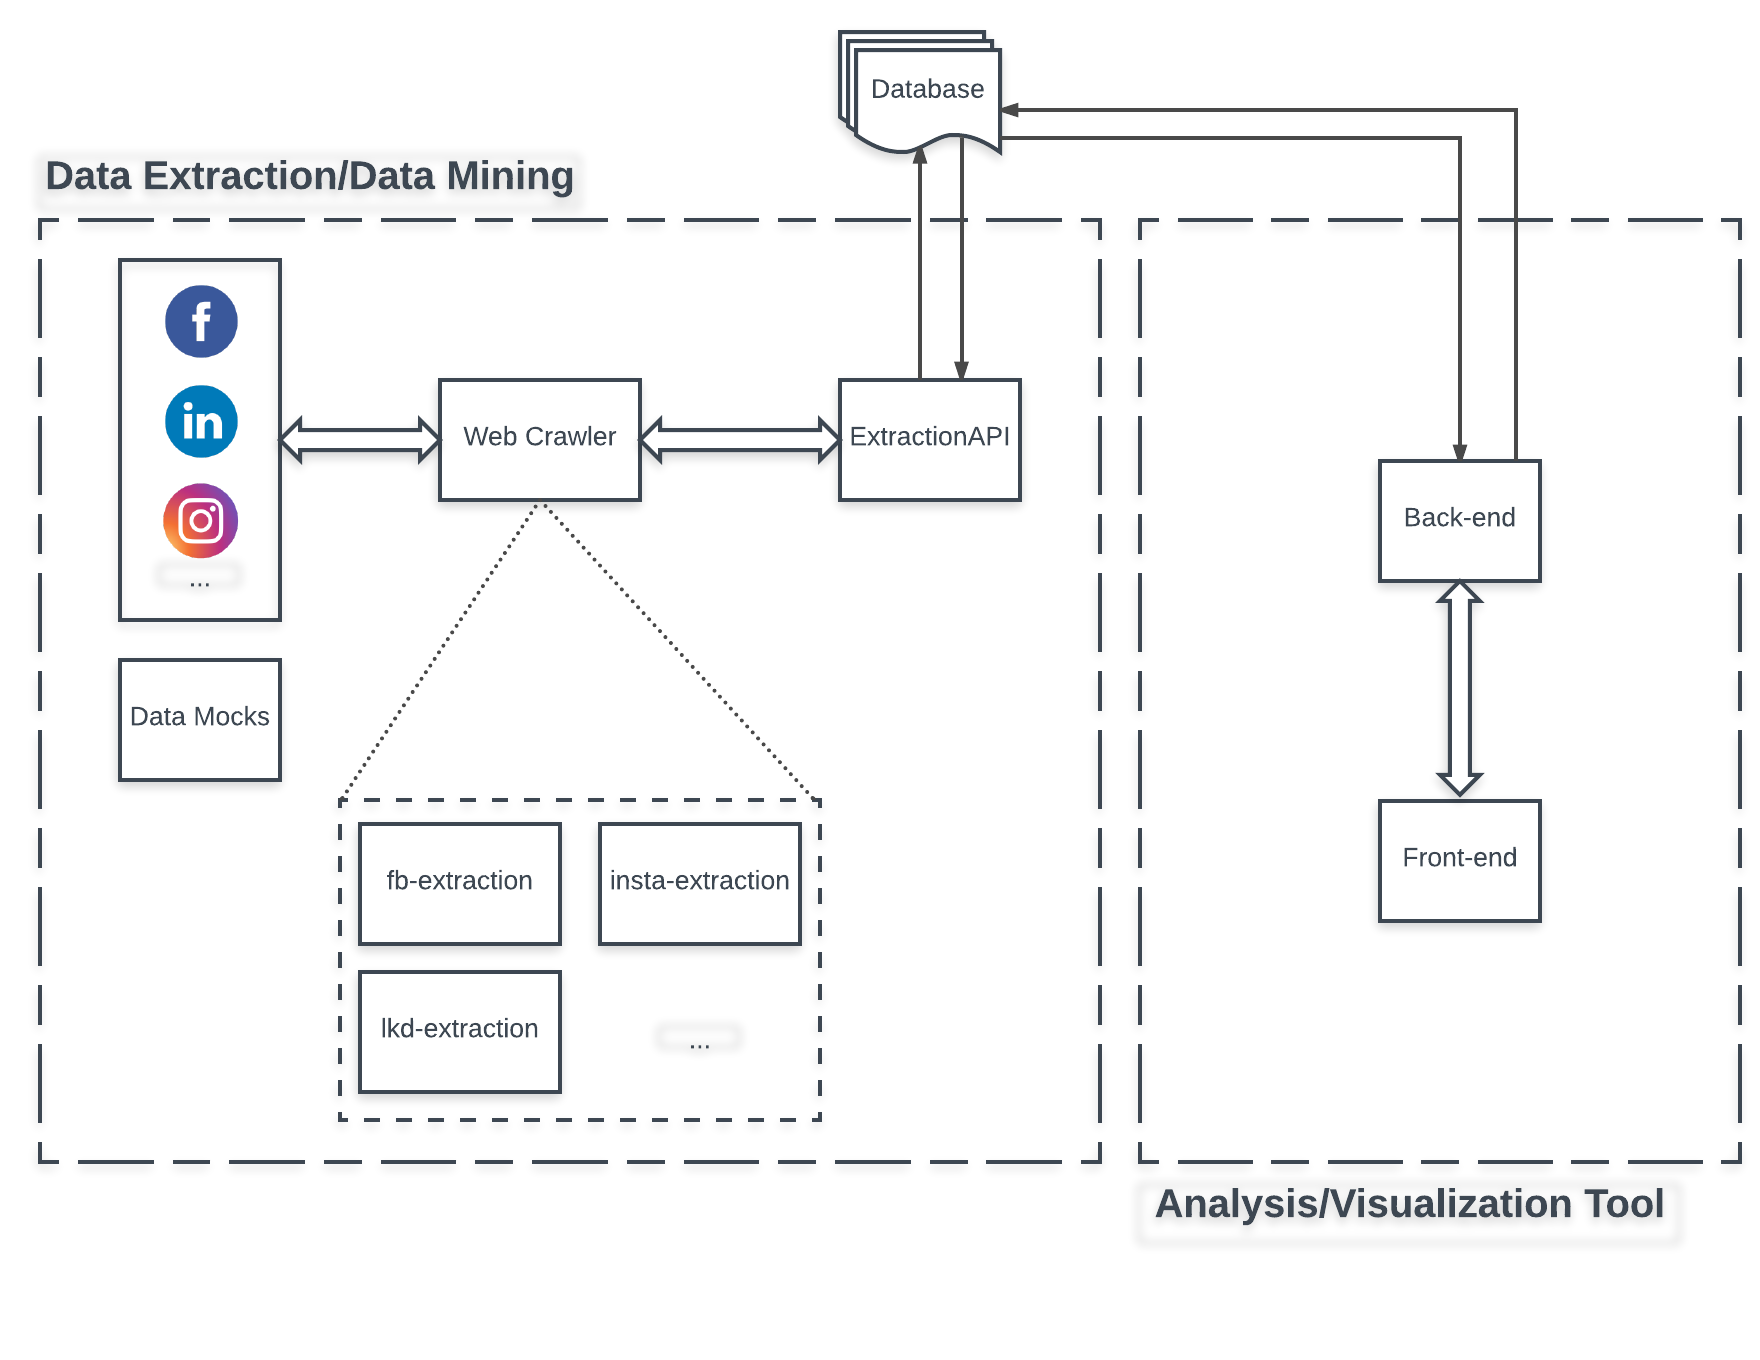
\includegraphics[width=1.1\textwidth]{img/architecture.png}
\end{center}
\caption{\label{img:architectureprop} System architecture proposal.}
\end{figure}

\subsection{General overview}
As the interaction of the software components may be clear from the diagram, the role of each module is not clear by simple
diagram observation, an underlying explanation of each component is needed in order to understand the system.\\
\indent We will follow a \textit{top down} approach for explaining the system architecture. First let us be clear about the two
main and distinct parts of the system:
\begin{itemize}
    \item \textbf{\textit{Information extraction and data mining}} - All the other components are built for extracting information
    from existent databases, or from \glspl{osn} (through the \textbf{Web Crawler}) and store information being information properly treated before stored;
    \item \textbf{\textit{Analysis and Application/Visualization}} - The tool that directly interacts with the end user is composed by a \textbf{Service Aggregator} that fetches data from a database, requests extractions to the application back-end and runs calculations and algorithms on top of stored networks as the user requests by interacting with a \textbf{Front-end} that provides the visualization and interaction features.
\end{itemize}


\subsection{Detailed Components Description}
The components presented in Figure \ref{img:architectureprop} more detailed explanation, next we look more carefully into each on of the components.
\begin{itemize}
    \item \textbf{\textit{\acrfull{osn}}} - This are the object of study, the source of information that the systems will process and analyze;
    \item \textbf{\textit{Web Crawler}} - The \textbf{Web Crawler} consists in a set of modules for crawling each one of the \glspl{osn} (\textit{fb-extraction} and other modules);
    \item \textbf{\textit{Data Miner}} - This module consists in a wrapper for extracting information from social networks, and allows extraction orchestration spreading extraction processes along multiple hosts, so that we can mitigate the slowness of web crawlers and extraction process in general. The data mining process is also implemented in this module assuring that we store a well defined data schema that describes in the more simplified way the state of the networks;
    \item \textbf{\textit{Database}} - The database is where we store our data. It is not represented by the \textit{classical cilindro} because it resembles relational databases, and the possibility of using non relational databases such as document databases, grows strongly within the project, and the reason is the unstructured data that we will be storing into our database. We also plan on feeding some data trough already existing databases, instead of crawling data from \gls{osn}. This databases may be provided from projects that we already mentioned in this document  (\hyperref[sec:otherdatasources]{Section 3.3.6}), such as \cite{kunegis2013konect}. This data would be accessed through the \textbf{Data Miner}, or a new module could be constructed exclusively to feed this data to our database;
    \item \textbf{\textit{Service Aggregator}} - Ideally this component application will read the already normalized information from the database, run \glspl{sna} calculations and algorithms against the stored networks, and request data to the back-end (the Information extraction and data mining super component);
    \item \textbf{\textit{Front-end}} - The front-end will render the networks to the user, and will allow the user to interact with the network; these interactions will be defined in the requirements specifications.
\end{itemize}
